\documentclass[letterpaper, reqno,11pt]{article}
\usepackage[margin=1.0in]{geometry}
\usepackage{color,latexsym,amsmath,amssymb,graphicx,float,listings,tikz}
\usepackage{hyperref}

\hypersetup{
colorlinks=true,
linkcolor=magenta,
filecolor=magenta,
urlcolor=cyan,
}

\graphicspath{ {images/} }

\begin{document}
\pagenumbering{arabic}
\title{PHYS 403 Problem Set 3}
\date{11/02/24}
\author{Xander Naumenko}
\maketitle

{\medskip\noindent\bf Question I1.} 
\[
H=mgz+\frac{1}{2}mv^2
.\]

{\medskip\noindent\bf Question I2.} Because the $v$ velocity term is independent of the height $z$, we can treat the Hamilton as $H=mgz$ (more precisely, the $e^{\frac{1}{2}mv^2}$ terms would cancel between the energy and partition function).
\[
p(z)= \frac{1}{Z}e^{-\beta mgz}= \frac{e^{-\beta mgz}}{\int_{0}^{\infty}e^{-\beta mgz'}dz'}
.\]

{\medskip\noindent\bf Question I3.} We can assume that density is proportional to the probability at a given elevation. Thus:
\[
\frac{p(z_{\text{Mt Everest}})}{p(z_{\text{Sea Level}})}=e^{-\beta mg(z_\text{Mt Everest}-z_\text{Sea Level})}=e^{-4.6528\cdot 10^{-26}\cdot 9.81\cdot 8848 /(270\cdot 1.381\cdot 10^{-23}}) = 0.34
.\]
This makes sense. According to Wikipedia the atmosphere pressure there is around 33.7kPa, which compared to atmospheric pressure of $101.325$kPA is a ratio of $0.33$ (which given we're assuming sea level and Mount Everest have the same temperature is surprisingly close).

{\medskip\noindent\bf Question II1.} Just summing over the possibilities explicitly:
\[
Z = e^{-\beta \cdot 0}+2e^{\beta \epsilon_b}+e^{-\beta(-2\epsilon_b+U)}
.\]

{\medskip\noindent\bf Question II2.} For the number of electrons, we can can compute the expected value, where $Z$ is defined as before:
\[
\langle \#\text{ Electrons} \rangle =\frac{1}{Z}\left( 2e^{\beta \epsilon_b}+2e^{-\beta(-2\epsilon_b+U)} \right) 
.\]
The plot of this function can be seen in figure \ref{fig:II2a}. Note that the question asks for graphs of temperature but specifies the range in terms of $k_BT$, so to keep the numbers nicer the $x$ axis is $k_BT$.

\begin{figure}[htpb]
    \centering
    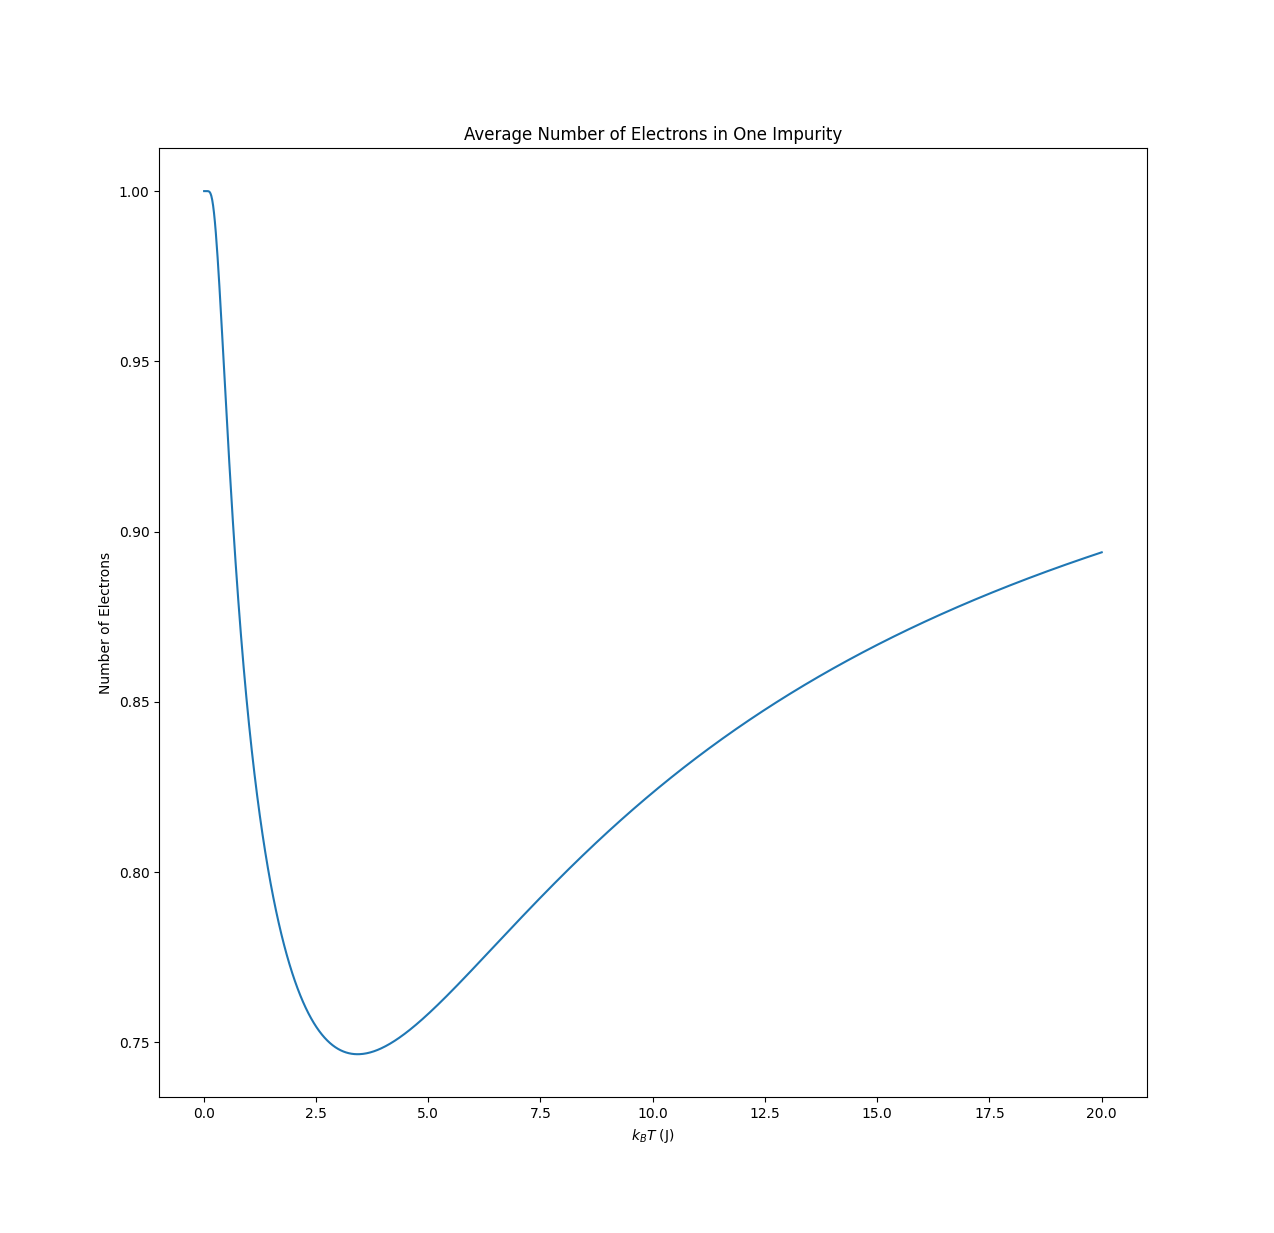
\includegraphics[width=0.8\textwidth]{II2a}
    \caption{Graph for question II2a.}
    \label{fig:II2a}
\end{figure}

Next for the energy, we can write out a similar expression, the graph is in figure \ref{fig:II2b}:
\[
\langle E \rangle =\frac{1}{Z}\left( -2\epsilon_b e^{\beta \epsilon_b}+(-2\epsilon_b+U)e^{-\beta(-2\epsilon_b+U)} \right) 
.\]

\begin{figure}[htpb]
    \centering
    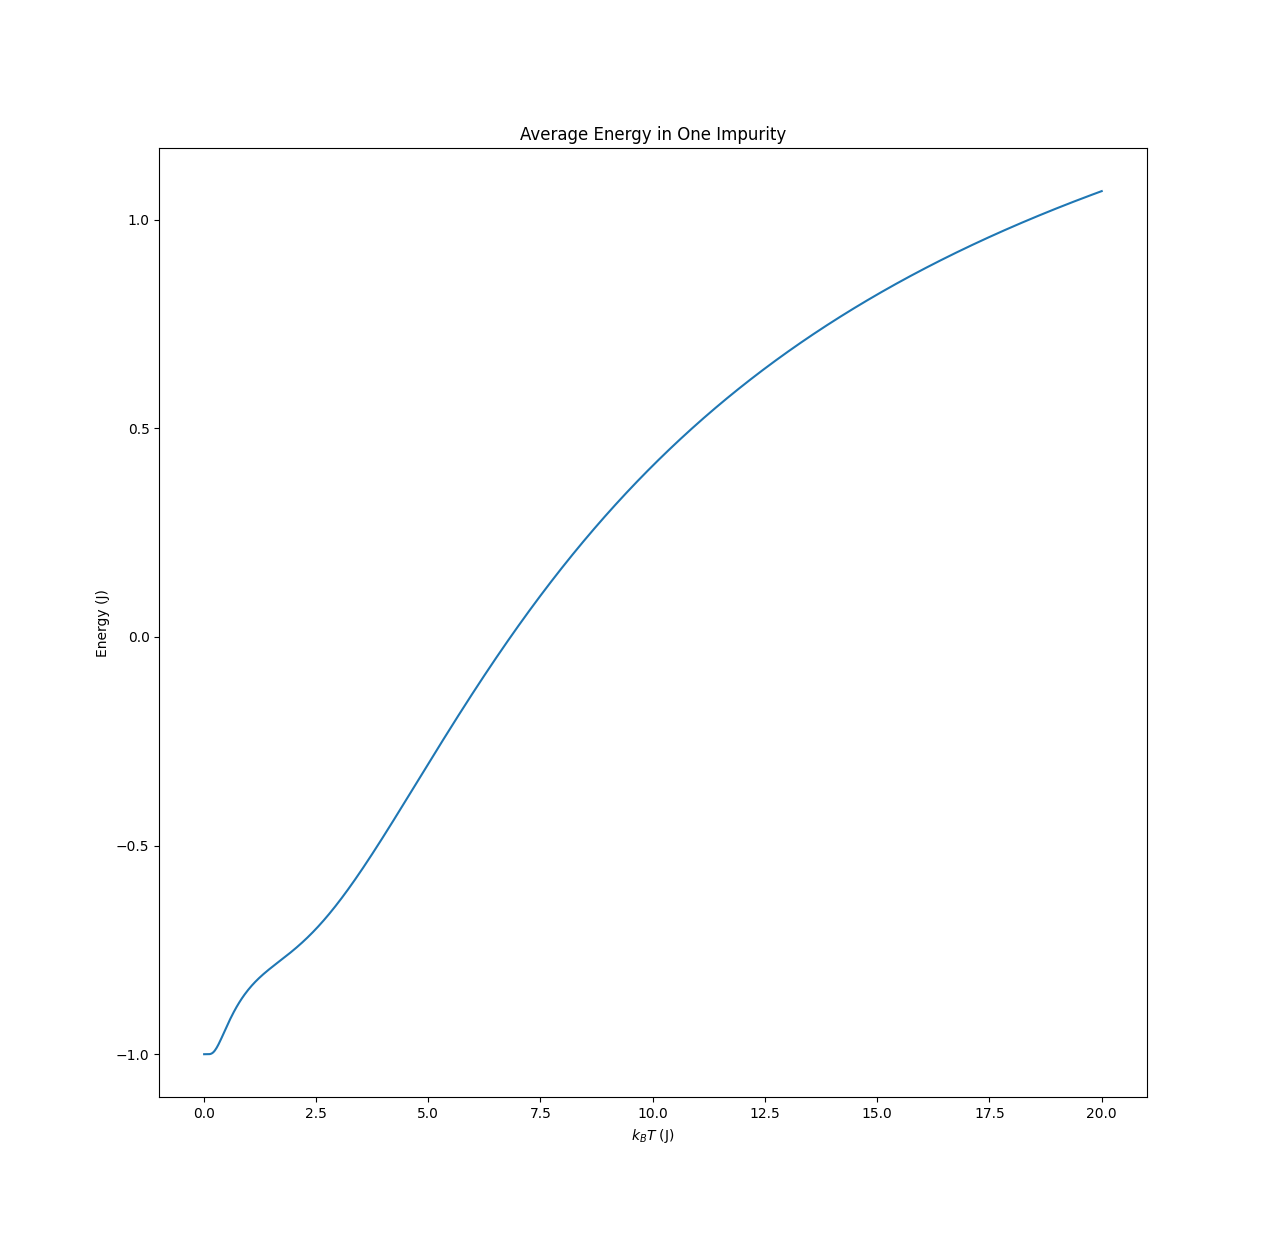
\includegraphics[width=0.8\textwidth]{II2b}
    \caption{Graph for question II2b}
    \label{fig:II2b}
\end{figure}

Finally, for heat capacity, we can find it in terms of $\langle E \rangle $:
\[
C = \frac{\partial \langle E \rangle }{\partial T}
.\]
Numerical differention was used to calculate this derivative in figure \ref{fig:II2c}, although in theory it would be a simple quotient rule application. Here is the code used:

\begin{figure}[htpb]
    \centering
    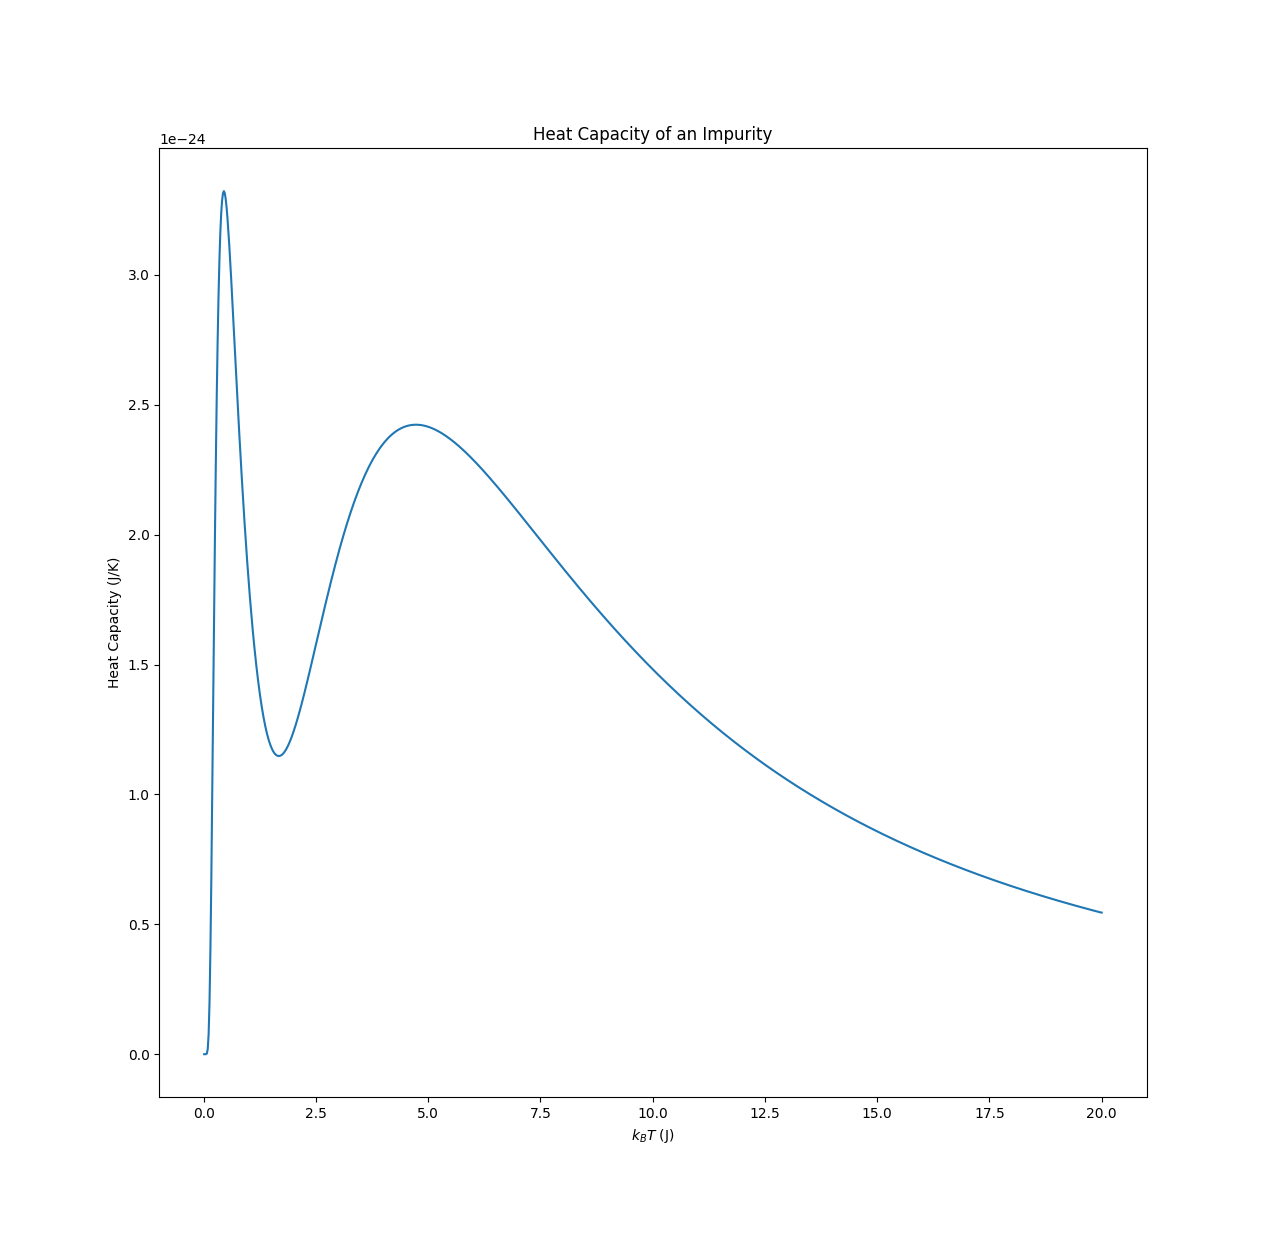
\includegraphics[width=0.8\textwidth]{II2C}
    \caption{Graph for question II2c}
    \label{fig:II2c}
\end{figure}

\begin{lstlisting}
import numpy as np
import matplotlib.pyplot as plt

eb = 1
U = 12
kb = 1.381e-23
T = np.linspace(0.01/kb, 20/kb, 1000)
dT = T[1] - T[0]

beta = 1/(kb*T)
Z = 1+2*np.exp(beta*eb)+np.exp(-beta*(-2*eb+U))


ne = 1/Z * (2*np.exp(beta*eb)+2*np.exp(-beta*(-2*eb+U)))

plt.plot(kb*T, ne)
plt.title("Average Number of Electrons in One Impurity")
plt.xlabel("$k_BT$ (J)")
plt.ylabel("Number of Electrons")
plt.show()

E = 1/Z * (-2*eb*np.exp(beta*eb)+(-2*eb+U)*np.exp(-beta*(-2*eb+U)))

plt.plot(kb*T, E)
plt.title("Average Energy in One Impurity")
plt.xlabel("$k_BT$ (J)")
plt.ylabel("Energy (J)")
plt.show()

C = np.gradient(E, dT)

plt.plot(kb*T, C)
plt.title("Heat Capacity of an Impurity")
plt.xlabel("$k_BT$ (J)")
plt.ylabel("Heat Capacity (J/K)")
plt.show()
\end{lstlisting}

{\medskip\noindent\bf Question III1.} All that's relevant here is the energy levels:
\[
Z = \sum_{n=0}^{\infty}e^{-\hbar\omega(n+1 /2)/(k_BT)}=e^{-\hbar\omega/(2k_BT)} \frac{1}{1-e^{-\hbar\omega /(k_BT)}}
.\]

{\medskip\noindent\bf Question III2.}
\[
\langle E \rangle = -\frac{\partial}{\partial \beta}\log Z=\frac{\hbar\omega}{2}+\frac{\partial}{\partial \beta}\log\left( 1-e^{-\beta\hbar\omega}\right)=\frac{\hbar\omega}{2}+ \frac{\hbar\omega}{e^{\beta\hbar\omega}-1}
.\]

{\medskip\noindent\bf Question III3.} 
\[
C=\frac{\partial}{\partial T}\langle E \rangle = \frac{(\hbar\omega)^2e^{\hbar\omega/(k_BT)}}{k_BT^2\left( e^{(\hbar\omega)/(k_BT)}-1 \right) ^2}
.\]


\end{document}
